\section*{Roofline Model (naive)}
\begin{minipage}{.6\linewidth}
  \flushleft
  \begin{itemize}
  \item max task-processing speed: \textcolor{red}{$P$ [flop/s]}
  \item bottleneck
    \begin{itemize}[label=-]
    \item execution of work: P$_{peak}$ [flop/s]
    \item data path: \textcolor{Green}{$I\cdot b_s$} [flop/byte $\cdot$ byte/s]
    \end{itemize}
  \end{itemize}
\[
\textcolor{red}{P} = \textsf{min}(\textcolor{Cyan}{P_{\text{peak}}}, \textcolor{Green}{I\cdot b_{s}})
\]
  \begin{itemize}
  \item High intensity: P limited by execution
  \item Low intensity: P limited by data transfer
  \item best use of resources (also max use of power): \textcolor{Tan}{Knee} at $P_{max} = I \cdot b_s$
  \item \textcolor{red}{roofline} is ``optimistic'' because it assumes data moves at \textcolor{red}{light speed}
  \end{itemize}
\end{minipage}
\begin{minipage}{.4\linewidth}
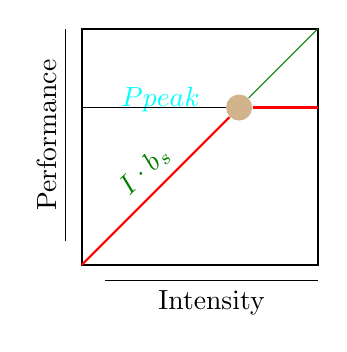
\begin{tikzpicture}
  % Knee
  \node[shape=circle,radius=1mm,fill=Tan]
  (knee) at (2,2) {};

  % Peaknode
  \node[color=Cyan] (peak) at (1,2.1) {$P\text{peak}$};

  % Ibsnode
  \node[color=Green,rotate=45] (ibs) at (.8,1.2)
  {$I\cdot b_s$};

  % rectangle coordinates
  \draw[thick] (0,0) rectangle (3,3);

  % y axis
  \draw (-.2, .3) edge[]
  node[above,sloped]{Performance} (-.2,3);

  % x axis
  \draw (.3, -.2) edge[]
  node[below]{Intensity} (3,-.2);

  % Peak
  \draw (0,2) -- (knee);
  \draw[color=red,thick] (knee) -- (3,2);

  % AI (I * Bs)
  \draw[color=red,thick] (0,0) -- (knee);
  \draw[color=Green] (knee) -- (3,3);

\end{tikzpicture}
\end{minipage}
